% Created by tikzDevice version 0.12.3.1 on 2022-09-01 15:58:50
% !TEX encoding = UTF-8 Unicode
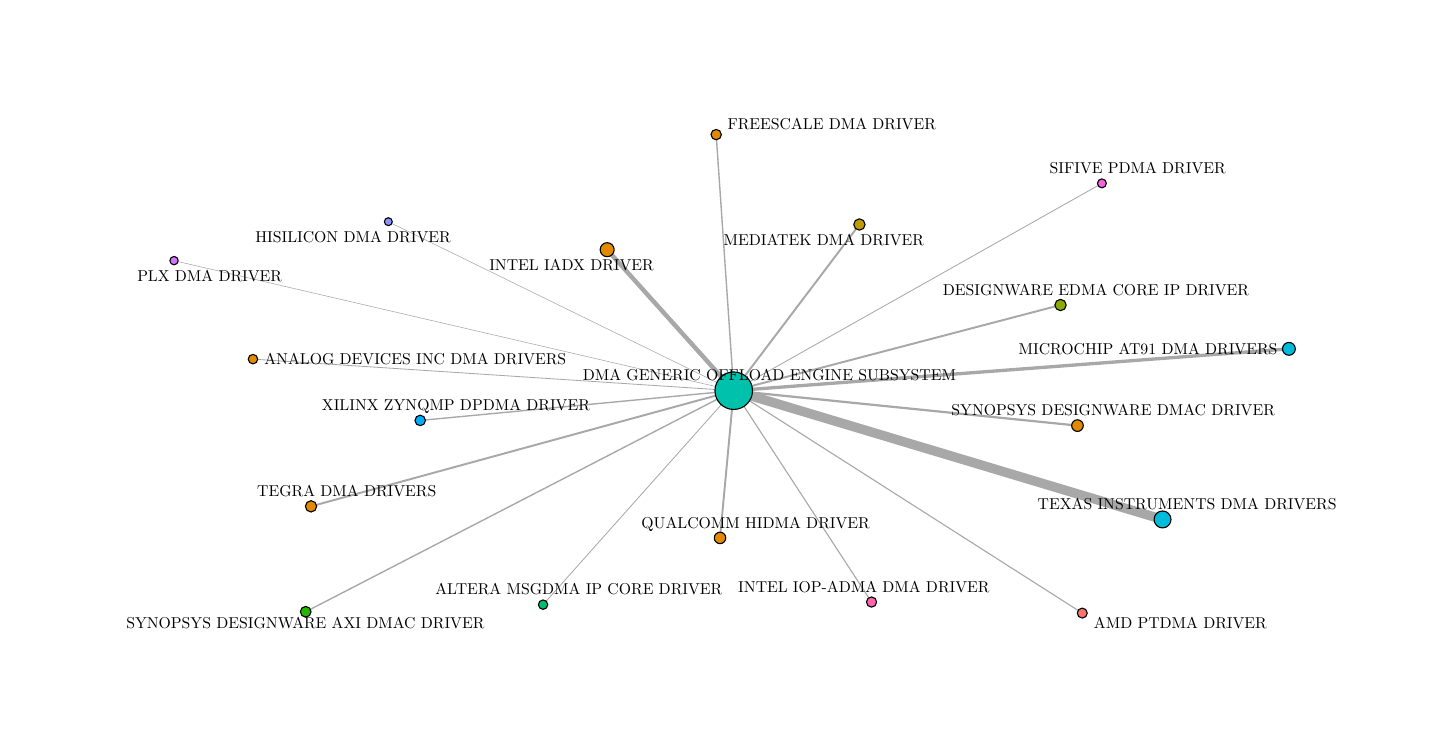
\begin{tikzpicture}[x=1pt,y=1pt]
\definecolor{fillColor}{RGB}{255,255,255}
\path[use as bounding box,fill=fillColor,fill opacity=0.00] (0,0) rectangle (505.89,252.94);
\begin{scope}
\path[clip] (  0.00,  0.00) rectangle (505.89,252.94);
\definecolor{fillColor}{RGB}{255,255,255}

\path[fill=fillColor] (  0.00,  0.00) rectangle (505.89,252.94);
\end{scope}
\begin{scope}
\path[clip] ( 32.75, 32.75) rectangle (475.89,222.94);
\definecolor{drawColor}{gray}{0.66}

\path[draw=drawColor,line width= 0.3pt,line join=round] (186.24, 44.45) -- (255.13,121.76);

\path[draw=drawColor,line width= 0.4pt,line join=round] (381.07, 41.40) -- (255.13,121.76);

\path[draw=drawColor,line width= 0.3pt,line join=round] ( 81.41,133.16) -- (255.13,121.76);

\path[draw=drawColor,line width= 0.7pt,line join=round] (373.22,152.72) -- (255.13,121.76);

\path[draw=drawColor,line width= 0.5pt,line join=round] (255.13,121.76) -- (248.79,214.30);

\path[draw=drawColor,line width= 0.2pt,line join=round] (255.13,121.76) -- (130.32,182.83);

\path[draw=drawColor,line width= 1.6pt,line join=round] (255.13,121.76) -- (209.40,172.71);

\path[draw=drawColor,line width= 0.4pt,line join=round] (255.13,121.76) -- (304.93, 45.39);

\path[draw=drawColor,line width= 0.7pt,line join=round] (255.13,121.76) -- (300.55,181.82);

\path[draw=drawColor,line width= 1.2pt,line join=round] (255.13,121.76) -- (455.75,136.88);

\path[draw=drawColor,line width= 0.2pt,line join=round] (255.13,121.76) -- ( 52.89,168.76);

\path[draw=drawColor,line width= 0.7pt,line join=round] (255.13,121.76) -- (250.18, 68.56);

\path[draw=drawColor,line width= 0.3pt,line join=round] (255.13,121.76) -- (388.17,196.68);

\path[draw=drawColor,line width= 0.5pt,line join=round] (255.13,121.76) -- (100.47, 41.88);

\path[draw=drawColor,line width= 0.8pt,line join=round] (255.13,121.76) -- (379.34,109.15);

\path[draw=drawColor,line width= 0.7pt,line join=round] (255.13,121.76) -- (102.39, 79.97);

\path[draw=drawColor,line width= 3.4pt,line join=round] (255.13,121.76) -- (410.08, 75.24);

\path[draw=drawColor,line width= 0.5pt,line join=round] (255.13,121.76) -- (141.84,111.01);
\definecolor{drawColor}{RGB}{0,0,0}
\definecolor{fillColor}{RGB}{0,190,112}

\path[draw=drawColor,line width= 0.4pt,line join=round,line cap=round,fill=fillColor] (186.24, 44.45) circle (  1.70);
\definecolor{fillColor}{RGB}{248,118,109}

\path[draw=drawColor,line width= 0.4pt,line join=round,line cap=round,fill=fillColor] (381.07, 41.40) circle (  1.80);
\definecolor{fillColor}{RGB}{225,138,0}

\path[draw=drawColor,line width= 0.4pt,line join=round,line cap=round,fill=fillColor] ( 81.41,133.16) circle (  1.71);
\definecolor{fillColor}{RGB}{140,171,0}

\path[draw=drawColor,line width= 0.4pt,line join=round,line cap=round,fill=fillColor] (373.22,152.72) circle (  2.05);
\definecolor{fillColor}{RGB}{0,193,171}

\path[draw=drawColor,line width= 0.4pt,line join=round,line cap=round,fill=fillColor] (255.13,121.76) circle (  6.78);
\definecolor{fillColor}{RGB}{225,138,0}

\path[draw=drawColor,line width= 0.4pt,line join=round,line cap=round,fill=fillColor] (248.79,214.30) circle (  1.87);
\definecolor{fillColor}{RGB}{139,147,255}

\path[draw=drawColor,line width= 0.4pt,line join=round,line cap=round,fill=fillColor] (130.32,182.83) circle (  1.43);
\definecolor{fillColor}{RGB}{225,138,0}

\path[draw=drawColor,line width= 0.4pt,line join=round,line cap=round,fill=fillColor] (209.40,172.71) circle (  2.53);
\definecolor{fillColor}{RGB}{255,101,172}

\path[draw=drawColor,line width= 0.4pt,line join=round,line cap=round,fill=fillColor] (304.93, 45.39) circle (  1.84);
\definecolor{fillColor}{RGB}{190,156,0}

\path[draw=drawColor,line width= 0.4pt,line join=round,line cap=round,fill=fillColor] (300.55,181.82) circle (  2.05);
\definecolor{fillColor}{RGB}{0,187,218}

\path[draw=drawColor,line width= 0.4pt,line join=round,line cap=round,fill=fillColor] (455.75,136.88) circle (  2.32);
\definecolor{fillColor}{RGB}{213,117,254}

\path[draw=drawColor,line width= 0.4pt,line join=round,line cap=round,fill=fillColor] ( 52.89,168.76) circle (  1.51);
\definecolor{fillColor}{RGB}{225,138,0}

\path[draw=drawColor,line width= 0.4pt,line join=round,line cap=round,fill=fillColor] (250.18, 68.56) circle (  2.07);
\definecolor{fillColor}{RGB}{249,98,221}

\path[draw=drawColor,line width= 0.4pt,line join=round,line cap=round,fill=fillColor] (388.17,196.68) circle (  1.61);
\definecolor{fillColor}{RGB}{36,183,0}

\path[draw=drawColor,line width= 0.4pt,line join=round,line cap=round,fill=fillColor] (100.47, 41.88) circle (  1.93);
\definecolor{fillColor}{RGB}{225,138,0}

\path[draw=drawColor,line width= 0.4pt,line join=round,line cap=round,fill=fillColor] (379.34,109.15) circle (  2.10);

\path[draw=drawColor,line width= 0.4pt,line join=round,line cap=round,fill=fillColor] (102.39, 79.97) circle (  2.04);
\definecolor{fillColor}{RGB}{0,187,218}

\path[draw=drawColor,line width= 0.4pt,line join=round,line cap=round,fill=fillColor] (410.08, 75.24) circle (  3.06);
\definecolor{fillColor}{RGB}{0,172,252}

\path[draw=drawColor,line width= 0.4pt,line join=round,line cap=round,fill=fillColor] (141.84,111.01) circle (  1.90);

\node[text=drawColor,anchor=base,inner sep=0pt, outer sep=0pt, scale=  0.57] at (199.16, 48.02) {ALTERA MSGDMA IP CORE DRIVER};

\node[text=drawColor,anchor=base,inner sep=0pt, outer sep=0pt, scale=  0.57] at (416.54, 35.76) {AMD PTDMA DRIVER};

\node[text=drawColor,anchor=base,inner sep=0pt, outer sep=0pt, scale=  0.57] at (140.07,131.22) {ANALOG DEVICES INC DMA DRIVERS};

\node[text=drawColor,anchor=base,inner sep=0pt, outer sep=0pt, scale=  0.57] at (386.04,156.25) {DESIGNWARE EDMA CORE IP DRIVER};

\node[text=drawColor,anchor=base,inner sep=0pt, outer sep=0pt, scale=  0.57] at (268.03,125.34) {DMA GENERIC OFFLOAD ENGINE SUBSYSTEM};

\node[text=drawColor,anchor=base,inner sep=0pt, outer sep=0pt, scale=  0.57] at (290.55,216.01) {FREESCALE DMA DRIVER};

\node[text=drawColor,anchor=base,inner sep=0pt, outer sep=0pt, scale=  0.57] at (117.55,175.37) {HISILICON DMA DRIVER};

\node[text=drawColor,anchor=base,inner sep=0pt, outer sep=0pt, scale=  0.57] at (196.52,165.22) {INTEL IADX DRIVER};

\node[text=drawColor,anchor=base,inner sep=0pt, outer sep=0pt, scale=  0.57] at (302.16, 48.99) {INTEL IOP-ADMA DMA DRIVER};

\node[text=drawColor,anchor=base,inner sep=0pt, outer sep=0pt, scale=  0.57] at (287.69,174.33) {MEDIATEK DMA DRIVER};

\node[text=drawColor,anchor=base,inner sep=0pt, outer sep=0pt, scale=  0.57] at (404.85,134.92) {MICROCHIP AT91 DMA DRIVERS};

\node[text=drawColor,anchor=base,inner sep=0pt, outer sep=0pt, scale=  0.57] at ( 65.76,161.27) {PLX DMA DRIVER};

\node[text=drawColor,anchor=base,inner sep=0pt, outer sep=0pt, scale=  0.57] at (263.04, 72.14) {QUALCOMM HIDMA DRIVER};

\node[text=drawColor,anchor=base,inner sep=0pt, outer sep=0pt, scale=  0.57] at (401.08,200.27) {SIFIVE PDMA DRIVER};

\node[text=drawColor,anchor=base,inner sep=0pt, outer sep=0pt, scale=  0.57] at (100.34, 35.76) {SYNOPSYS DESIGNWARE AXI DMAC DRIVER};

\node[text=drawColor,anchor=base,inner sep=0pt, outer sep=0pt, scale=  0.57] at (392.24,112.71) {SYNOPSYS DESIGNWARE DMAC DRIVER};

\node[text=drawColor,anchor=base,inner sep=0pt, outer sep=0pt, scale=  0.57] at (115.30, 83.53) {TEGRA DMA DRIVERS};

\node[text=drawColor,anchor=base,inner sep=0pt, outer sep=0pt, scale=  0.57] at (418.98, 78.82) {TEXAS INSTRUMENTS DMA DRIVERS};

\node[text=drawColor,anchor=base,inner sep=0pt, outer sep=0pt, scale=  0.57] at (154.75,114.60) {XILINX ZYNQMP DPDMA DRIVER};
\end{scope}
\end{tikzpicture}
